\begin{figure}[h]
    \centering
    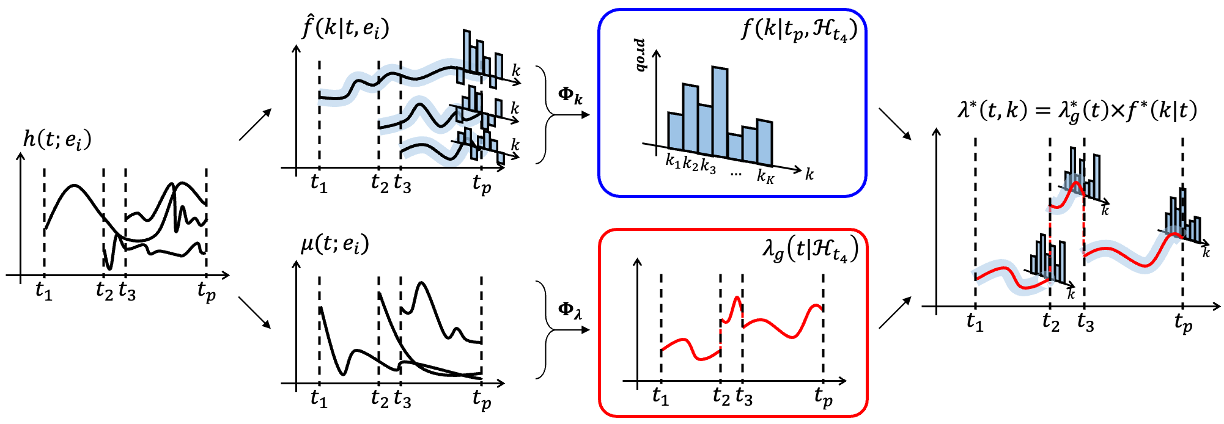
\includegraphics[width=0.95\linewidth]{figure/main_figure_final.png}
    \caption{\small A visualization of the overall framework. Hidden states from each event $e_i$ are independently propagated and decoded into trajectories of $\mu(t;e_i)$ and $\hat{f}_k (k|t, e_i)$. Each trajectory represents the effect of each event on the MTPP, and the MTPP can be reconstructed by combining all trajectories.}
    % \vspace{-10pt}
    \label{fig:main}
    % \vspace{-5pt}
\end{figure}

\section{Decoupling Marked Time Point Process}
Our approach focuses on establishing a general framework that captures the high-fidelity distribution of MTPP with decoupled structures. 
Specifically, given a sequence of events denoted as $\mathcal{S} = \{e_i\}_{i=0} ^n$
, where an event $e_i = (t_i, k_i)$ is composed of a time point and a marker, with $n+1$
observed events, our goal is to predict a probability distribution of an event $e_{n+1}$. 
Unlike previous works that directly estimate the conditional intensity $\lambda^*(t,k)$, we take an alternative approach of 
separately estimating the ground intensity and the distribution of event, i.e., $\lambda _g ^*(t)$ and $f^*(k|t)$. 

In our framework, the influences from each events through time are represented by hidden state dynamics $h(t;e_i)$, which  
undergo a decoding process 
to yield $\lambda ^*_g(t)$ and $f^*(k|t)$ separately. As described in Fig.\ref{fig:main}, $\lambda^* _g(t)$ and $f^*(k|t)$ form independent trajectories, and they are combined in the later stage to constitute $\lambda^*(t,k)$.


\subsection{Hidden State Dynamics \label{continuous modeling}} 

In this section, we introduce decoupled hidden state dynamics, 
where the hidden state is used to characterize the influence each event $e_i$ has on the overall process.

The decoupled hidden states $h(t; e_i) \in \mathbb{R}^d$, where $i=1, \cdots, n$,
are independently propagated through time from the occurrence of each event at $t_i$.  
The dynamics of $h(t; e_i)$, which will be used to characterize the complex dynamics of the intensity function within MTPP, are trained using the Neural ODEs \cite{bib:node}. 

Specifically, the initial magnitude of a hidden state $h(t_i;e_i)$ depends on the event type $k_i$, 
and the 
dynamics are solved via initial value problem (IVP) solvers. 
Then the hidden state caused by an event $e_i$ at time $t$ can be obtained as: 
\begin{align}
d h(t;e_i) &=  \gamma(h(t;e_i), t, k_i;\theta) dt \\
h(t;e_i) &= h(t_i;e_i) + \int ^t _{t_i} \gamma(h(s;e_i), s, k_i;\theta) ds \nonumber\\
& = W_{e}(k_i) + \int ^t _{t_i} \gamma(h(s;e_i), s, k_i;\theta) ds 
\label{eq:hiddenS}
\end{align}
where the initial magnitude is obtained using $W_{e}(\cdot): \{1, \cdots, K\} \rightarrow \mathbb{R}^{d}$, which is trainable, and $\gamma$ is parameterized with a neural network $\theta$. Hidden states at time $t$ can be computed in parallel as a multidimensional ODE by 
taking advantages of the decoupled structure of $h(t;e_i)$ as 
\begin{align}
    {d \over dt} \mathbf{h(t)} = 
    {d \over dt}
    \begin{bmatrix}
        h(t;e_0) \\
        \vdots \\ h(t;e_i)
    \end{bmatrix}
    = 
    \begin{bmatrix}
        \gamma(h(t;e_0), t, k_0;\theta) \\ \vdots \\ \gamma(h(t;e_i), t, k_i; \theta)
    \end{bmatrix}. 
    \label{eq: hidden parallel}
\end{align}
One major advantage of the decoupling is that the influence of events from $\mathbf{h}(t)$ can be selectively considered. 
For example, when computing $f^*(t)$ 
conditioned on $\mathcal{H}_{t_j}$, where $t > t_{j+1}$, $h(t;e_{t_{j+1}})$ should not be included in computation. The details will be discussed in the Sec. \ref{sec:ground int}.

\subsection{Ground intensity function \label{sec:ground int}}

In our method, the ground intensity $\lambda _g ^*(t)$ is defined as a mixture of decoupled \textit{influence functions} $\mu(t;e_i)$, which can be considered as a generalized form of the exciting functions found in the Hawkes process \cite{bib:hawkes}. 
Since each influence function is conditioned on a single event, in order to define $\lambda _g (t|\mathcal{H}_t)$, i.e., the ground intensity conditioned on the history, the influences from historical events must be aggregated. 
The conditional ground intensity function is defined as,
\begin{align}
    \lambda_g(t|\mathcal{H}_{t_{n+1}}) =\lambda_g(t|e_0, \cdots, e_n) = \Phi_\lambda(\mu(t;e_0), \cdots, \mu(t;e_n))
    \label{eq:lambdag}
\end{align}
where $\mu(t;e_i) := g_\mu(h(t;e_i))$ is decoded by a neural network $g_\mu : \mathbb{R}^d \rightarrow \mathbb{R}$, $ e_i \in \mathcal{H}_{t_{n+1}}$ is an observed event, and $\Phi_\lambda$ is a positive function to satisfy the non-negativity constraints of $\lambda ^* _g (t)$. 
Notice that the hidden state $h(t;e_i)$ is decoded into the influence function $\mu(t;e_i)$ before aggregated into $\lambda ^*_g(t)$, otherwise, influence from a specific event would not be observable. 



When learning a TPP, integration is pivotal. Not only does the computation of probability distribution $f ^*(t):= \lambda^*(t) \exp(-\int _{t_{i-1}} ^t \lambda^* (s) ds)$ requires an integration, but also obtaining characteristic functions, survival rate, etc. requires additional integration 
which does not have a closed-form solution in general. 
Therefore, intensity-based methods often require additional steps for predictions. 
Methods such as Monte Carlo Inference \cite{bib:nhp, bib:sahp, bib:THP, bib:ANHP} are often used for calculating $f^*(t)$, 
while sampling methods such as the thinning algorithm \cite{bib:nhp} are adopted for computing the expected value. 
In these approaches, each integration has to be handled separately with additional sampling.
The Neural ODEs, which we extensively utilize to solve for the MTPP, 
is inherently computationally heavier compared to Monte Carlo Inference due to its sequential solving mechanism. 
To circumvent the extra computational burden, we leverage the characteristics of the differential equation. 
By simultaneously solving the following multi-dimensional differential equation with respect to $\mathbf{h}(t)$ along with numerical integration, we eliminate the need for additional sampling: 
\begin{align}
\label{eqn:multi-integral}
{\partial \over \partial t} 
\begin{bmatrix}
\mathbf{h}(t) \\[1.5ex] 
\Lambda_g (t |  \mathcal{H}_{t_i}) \\[1.5ex] 
F(t | \mathcal{H}_{t_i}) \\[1.5ex] 
\mathbb{E}[t]
\end{bmatrix}
= 
\begin{bmatrix}
\gamma (\mathbf{h}(t),t, \mathbf{k}; \theta) \\[1.5ex] 
\lambda_g(t | \mathcal{H}_{t_i}) \\[1.5ex] 
f(t|\mathcal{H}_{t_i}) \\[1.5ex] 
t \cdot f(t|\mathcal{H}_{t_i})
\end{bmatrix}
= 
\begin{bmatrix}
\gamma (\mathbf{h}(t),t,\mathbf{k}; \theta) \\[1.5ex] 
\Phi_\lambda( g_\mu(\mathbf{h}(t))) \\[1.5ex] 
\lambda_g(t|\mathcal{H}_{t_i}) \cdot \exp (\Lambda_g(t_{i-1}|\mathcal{H}_{t_i}) - \Lambda_g(t|\mathcal{H}_{t_i}) ) \\[1.5ex] 
t \cdot f(t|\mathcal{H}_{t_i}) 
\end{bmatrix}
\end{align}

where $\Lambda_g (t|\mathcal{H}_{t_i}) := \int ^t _0 \lambda_g (t | \mathcal{H}_{t_i}) dt$ is called the \textit{compensator}, and $\mathbf{k}$ is the marks corresponding to $\mathbf{h}(t)$. Because the dynamics are learned through differential equations, values at time $t$ can be used for computing others. e.g., $\lambda^*_g(t)$, which is a derivative of $\Lambda^*_g(t)$, can be computed using $\mathbf{h}(t)$.

\begin{wrapfigure}{r}{0.52\textwidth}
% \vspace{-5pt}
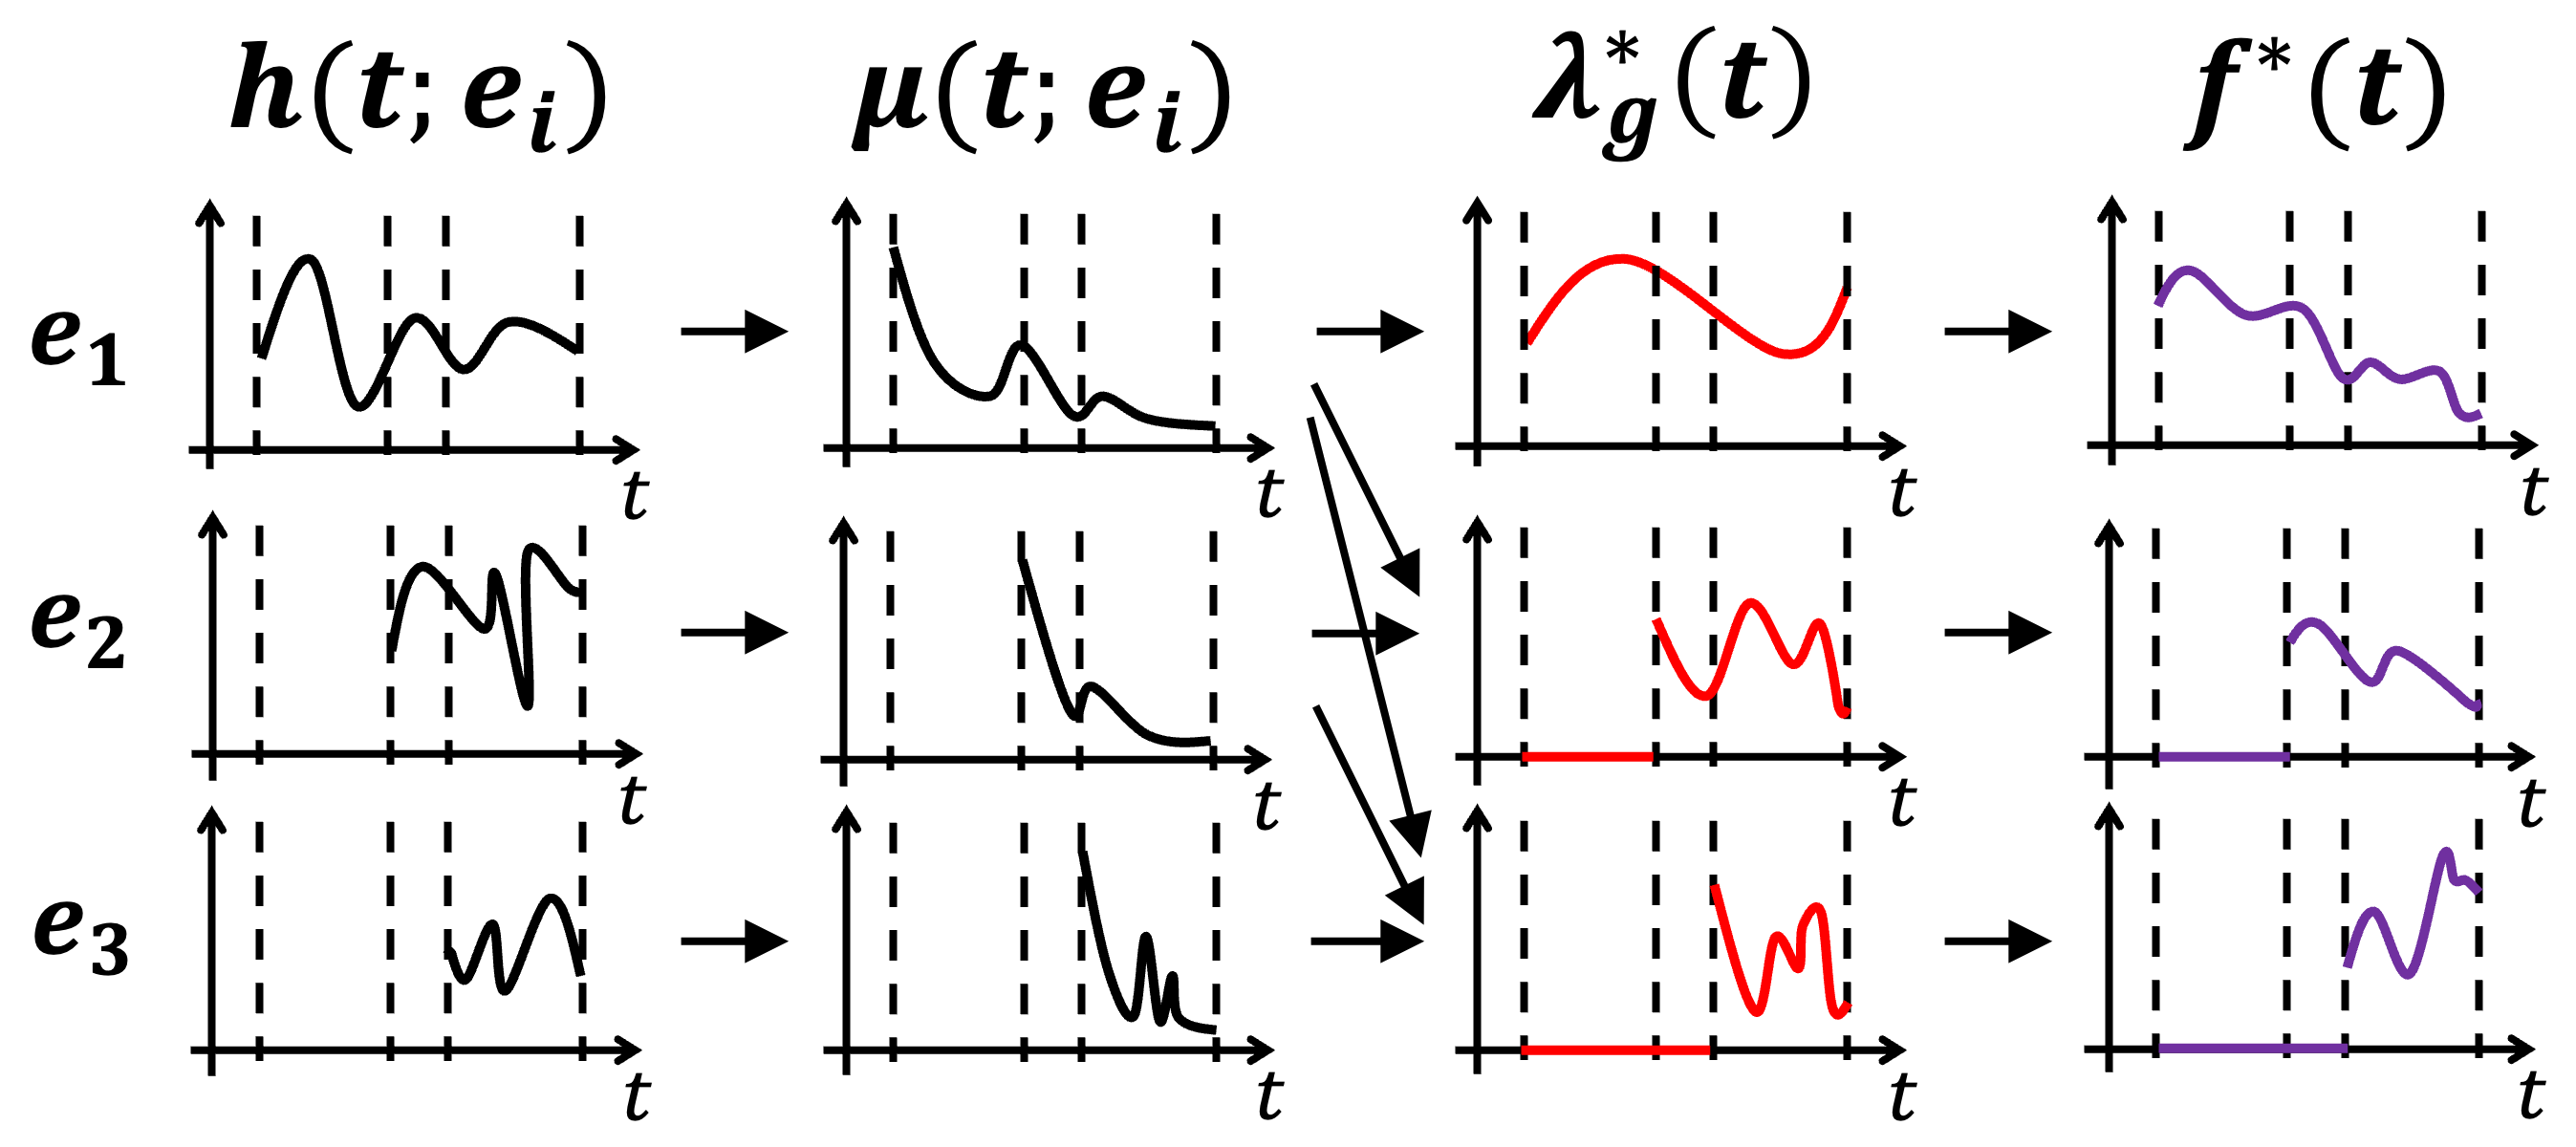
\includegraphics[width=0.50\textwidth]{figure/eq_9_figure2.png}
\captionsetup[figure]{font=small}
% \vspace{-3pt}
\caption{\small Visualization of \eqref{eqn:multi-integral}. Different combinations of $\mu(t;e_i)$ can be selected for calculating $\lambda ^*_g(t)$ and $f^*(t)$ conditioned on different $\mathcal{H}_{t_i}$ in parallel.}
% \vspace{-15pt}
\label{fig: selective DE}
\end{wrapfigure} 
Therefore, important estimations with integration, such as likelihood, survivor rate $S ^* (t) := 1- F^*(t)$, 
and $\mathbb{E}_{f^*} [t]$ can be predicted in a single run. 
This formulation can be applied to any number of integrations.
Moreover, as briefly mentioned in Sec. \ref{continuous modeling}, the influence functions can be selected according to our interests as illustrated in Fig. \ref{fig: selective DE}. 
Therefore, approximations of functions in \eqref{eqn:multi-integral} under different $\mathcal{H}_{t_i}$ can be obtained in parallel, distinguishing Dec-ODE from other intensity-based methods that require separate runs. 

% \vspace{-5pt}
\subsection{Conditional Probability for Marks \label{sec:fk}}
% \vspace{-5pt}

Similar to the formulation of the ground intensity in \eqref{eq:lambdag}, the probability of marks $f^* (k|t)$ can be expressed using the following form: 
\begin{equation}
 f(k|t, \mathcal{H}_{t_{n+1}}) = \Phi _k( \hat{f}(k|t,e_0), \cdots, \hat{f}(k|t,e_{n}))
 \end{equation}
where $\hat{f}(k|t,e_i):= g_f(h_t(e_i))$ is an influence from $e_i$ on $f(k|t)$, decoded by a neural network $g_f(\cdot)$. The function $\Phi_k$ combines $\hat{f}(k|t,e_i)$ over events while satisfying $\sum _K \Phi_k(\cdot)  = 1$. 

The intuition behind such a modeling is that the context of an event changing over time carries important information. For instance, getting a driver's license would dramatically increase the probability of causing a car accident since there was no chance without the license. 
However, as time goes on, the person gets better at driving and the probability decreases. 
Using the proposed structure, the changes of implications through time can be inferred by $\hat{f}(k|t_i,e_i)$.

 
\section{Linear Dec-ODE \label{Linear Decode}}

The combining functions $\Phi_\lambda$ and $\Phi_k$ can be chosen from a simple summation to a complex neural networks, such as Transformer. 
Nonetheless, in the following section, we present 
a linear version of Dec-ODE as it offers efficiency and interpretability via parallel modeling of the hidden states. 


\subsection{Combining Influences from Past Events}
In order to demonstrate the competence of the proposed framework, the implementation of $\Phi_\lambda$ and $\Phi_k$ is defined as linear and simple equations that combines influences of historical events for $\lambda ^* _g(t)$ and $f^*(k|t)$. 
The ground intensity $\lambda^* _g (t)$ and the conditioned probability of marks $f^*(k|t)$ are defined as combinations of decoupled dynamics :
\begin{equation}
\begin{aligned}
\lambda _g (t| \mathcal{H}_{t_{n+1}}) = \Phi_\lambda(\mu(t;e_0), \cdots, \mu(t;e_n)) = \sum _{e_i \in \mathcal{H}_{t_{n+1}}} \text{softplus} (\mu  (t; e_i))
\end{aligned}
\label{eq: lin-ground}
\end{equation}
\begin{equation}
\begin{aligned}
f(k|t, \mathcal{H}_{t_{n+1}}) = \Phi _k( \hat{f}(k|t,e_0), \cdots, \hat{f}(k|t,e_n)) = \text{softmax} \bigg( \sum_{e_i \in \mathcal{H}_{t_{n+1}}} \hat{f}(k|t,e_i)\bigg)
\end{aligned}
\end{equation}
where softplus and softmax functions are used to satisfy the constraints from Sec. \ref{sec:ground int} and Sec. \ref{sec:fk}, respectively.
This modeling of $\lambda^*_g(t)$ with linear summation resembles with the Hawkes process. 
Yet, our method can model more flexible temporal dynamics, and better suited for modeling complex real-life scenarios. 
 
%  \vspace{-5pt}
\subsection{Training Objective \label{sec:obj}}
% \vspace{-5pt}
The objective of our method is to maximize the likelihood of the predicted Marked TPP \cite{bib:daley}. 
Taking a $\log$ on the likelihood in \eqref{eq:likelihood}, 
\begin{equation}
\begin{aligned}
\ln f(t,k) &= \ln  \bigg[\prod ^{\mathcal{N}_g(t_N)} _{i=1} \lambda ^* _g (t_i)\bigg]\bigg[\prod ^{\mathcal{N}_g(t_N)} _{i=1} f ^* (k_i | t_i) \bigg] \exp \bigg( - \int ^{t_N} _0 \lambda ^*_g (u) du \bigg) \\
 &= \underbrace{\sum ^{\mathcal{N}_g(t_N)} _{i=1} \ln \lambda ^* _g (t_i) -   \int ^{t_N} _0 \lambda ^*_g (u) du}_{\ln L_\lambda} + \underbrace{\sum ^{\mathcal{N}_g(t_N)} _{i=1} \ln f ^* (k_i | t_i)}_{\ln L_k}
\label{eq:obj}
\end{aligned}
\end{equation}
where $t_N$ is the last observed time point, and the log-likelihood for the ground intensity $\ln L_\lambda$ and the mark distribution $\ln L_k$ are independently defined,
and used to learn $\lambda_g(t)$ and $f(k|t)$, respectively.
Intuitively, the first term in $L_\lambda$ is the probability of event happening at each $t_i$ and the second term is the probability of event not happening everywhere else. 
Therefore, $\lambda^*_g(t)$ should be high at the time of event's occurrence and low everywhere else to maximize $L_\lambda$.
Also, for the estimations, $f(t)$ is normalized to satisfy $\int f(t) dt = 1$.

% \vspace{-5pt}
\subsection{Training Scheme \label{train_parallel}}
% \vspace{-5pt}
Many previous works using differential equation based modeling \cite{bib:NJSDE, bib:STPP} 
sequentially solve the entire time range, which require  
exhaustive training time. 
In our case, using the characteristics of $\Phi_\lambda$ with linear summation, such limitation can be alleviated as follows. 

First, because each $\mu(t; e_i)$ is independent from other events, we can propagate them simultaneously as a multi-dimensional differential equation as
\begin{equation}
    d 
    \begin{bmatrix}
        \mu(\tau_0 ;e_0) \\ \vdots \\ \mu(\tau_i;e_i)
    \end{bmatrix}
    = 
    \begin{bmatrix}
        \gamma(\mu(\tau_0), \tau_0, k_0;\theta) \\ \vdots \\ \gamma(\mu(\tau_i), \tau_i, k_i; \theta)
    \end{bmatrix}
    \cdot d \boldsymbol{\tau}
    \label{eq: train_parallel}
\end{equation}
where $ \boldsymbol{\tau} =[\tau_0, \cdots, \tau_i] ^\top = [t_0 + t, t_1 + t, \cdots, t_i + t] ^ \top$. 

Second, one of the benefits of formulating the ground intensity as a linear equation is that 
the compensator $\Lambda^* _g(t)$ can also be calculated in the same manner as in \eqref{eq: lin-ground}
\begin{align}
    \Lambda^* _g (t)  & = \int _0 ^t \lambda_g ^* (s) ds = \int_0 ^t \sum _{e_i \in \mathcal{H}_{t}} \text{softplus} (\mu  (s; e_i)) ds \\    
    & = \sum_{e_i \in \mathcal{H}_{t}} \int _{t_i} ^t \text{softplus}( \mu (s; e_i)) ds
    \label{eq:Lambda}
\end{align}
where the region of the integration changes since there is no influence of $e_i$ before $t_i$.
The \eqref{eq:Lambda} conveys that the integration in \eqref{eq:obj} can be computed by integrating softplus
$(\mu(t;e_i))$ individually first and sum up later, 
instead of sequentially going through the entire sequence. 
Hence, if we can find the number of time-points $m$, we can solve the entire trajectory within a fixed number of steps. The effectiveness of such modeling is discussed in Sec. \ref{ablation: parallel}.